% concatenated from Hadamard_main.tex

\documentclass[12pt]{amsart}

\usepackage{amsmath,amssymb}
\usepackage{tikz}
\usepackage{graphicx}
\usepackage{float}
\usetikzlibrary{positioning,calc}
\usepackage{comment}
\usepackage{siunitx}
\usepackage{array} % needed for m{ } column types
\usepackage{url}
\usepackage{hyperref}
\usepackage{a4wide}

%\graphicspath{ {./} }

\newcommand{\md}{{\rm d}}
\newcommand{\dx}{\, \md x}
\newcommand{\dy}{\, \md y}
\newcommand{\drho}{\, \md \rho} 
\newcommand{\dphi}{\, \md \phi} 
\newcommand{\dtheta}{\, \md \theta} 
\newcommand{\dz}{\, \md z}
%\newcommand{\O}{\Omega}

\newcommand{\ds}{\displaystyle}
\let \l =\lambda


%JB macros
\newcommand{\er}{\mathbf{e}_{R}}
\newcommand{\et}{\mathbf{e}_{\theta}}
\newcommand{\bx}{\mathbf{x}}
\newcommand{\br}{\mathbf{r}}
\newcommand{\R}{\mathbb{R}}
\newcommand{\N}{\mathbb{N}}
\newcommand{\C}{\mathbb{C}}
\newcommand{\sC}{\scriptscriptstyle{\mathbb{C}}}
\newcommand{\half}{\frac{1}{2}}
\newcommand{\ep}{\varepsilon}
\newcommand{\om}{\Omega}
\newcommand{\Div}{{\rm div}\,}
\newcommand{\curl}{{\rm curl}\,}
\newcommand{\cof}{{\rm cof}\,}
\newcommand{\adj}{{\rm adj}\,}
\newcommand{\ul}{u_{\lambda}}
\newcommand{\un}{u_{_N}}
\newcommand{\unp}{u_{N}^{\scriptscriptstyle{\varphi}}}
\newcommand{\unpj}{u_{N}^{\scriptscriptstyle{\varphi^{(j)}}}}
\newcommand{\1}{{\bf 1}}
\newcommand{\tr}{{\rm tr}\,}
\newcommand{\eps}{\epsilon}
\newcommand{\scc}{\mathcal{C}}
\newcommand{\sca}{\mathcal{A}}
\newcommand{\scv}{\mathcal{V}}
\newcommand{\scu}{\mathcal{U}}
\newcommand{\sch}{\mathcal{H}}
\newcommand{\dist}{\textrm{dist}\,}
\newcommand{\scl}{\mathcal{L}}
\newcommand{\Det}{\mathrm{Det}\,}
\newcommand{\Per}{\mathrm{Per}\,}
\newcommand{\im}{\mathrm{im}\,}
\newcommand{\lam}{\lambda}
\newcommand{\scg}{\mathcal{G}}
\newcommand{\rb}{\bar{\rho}}
\newcommand{\rast}{\rho^{\ast}}
\newcommand{\atr}{\rm{atr}}
\newcommand{\scf}{\mathcal{F}}
\newcommand{\meas}{\textrm{meas}\,}
\newcommand{\spt}{\textrm{spt}\,}
\newcommand{\bt}{\bar{\theta}}
\newcommand{\ka}{\kappa}
\newcommand{\bw}{\bar{w}}
\newcommand{\hx}{\hat{x}}
\newcommand{\hy}{\hat{y}}
\newcommand{\hvarphi}{\hat{\varphi}}
\newcommand{\hphi}{\hat{\phi}}
\newcommand{\id}{\textrm{id}}
\newcommand{\pcr}{\psi|_{C_r}}
\newcommand{\D}{\mathbb{D}}
\newcommand{\bbi}{\mathbb{E}}
\newcommand{\pe}{p_{\eps}}
\newcommand*{\lc}{\mbox{\large$\chi$}}% big chi
\newcommand*\Laplace{\mathop{}\!\mathbin\bigtriangleup}%laplacian
\newcommand{\tv}{\tilde{v}}
\newcommand{\tphi}{\tilde{\phi}}
\newcommand{\tpsi}{\tilde{\psi}}
\newcommand{\re}{\mathrm{Re\,}}
\newcommand{\wto}{\rightharpoonup}

\def\Xint#1{\mathchoice
   {\XXint\displaystyle\textstyle{#1}}%
   {\XXint\textstyle\scriptstyle{#1}}%
   {\XXint\scriptstyle\scriptscriptstyle{#1}}%
   {\XXint\scriptscriptstyle\scriptscriptstyle{#1}}%
   \!\int}
\def\XXint#1#2#3{{\setbox0=\hbox{$#1{#2#3}{\int}$}
     \vcenter{\hbox{$#2#3$}}\kern-.5\wd0}}
\def\ddashint{\Xint=}
\def\dashint{\Xint-}

\newtheorem{definition}{Definition}[section]
\newtheorem{lemma}[definition]{Lemma}
\newtheorem{theorem}[definition]{Theorem}
\newtheorem{proposition}[definition]{Proposition}
\newtheorem{corollary}[definition]{Corollary}
\newtheorem{remark}[definition]{Remark}
\newtheorem{conjecture}[definition]{Conjecture}

% JHBD macro
\renewcommand{\rb}{\raisebox{2.7ex}{}}
%\renewcommand{\restriction}{\mathord{|}}
\newcommand\EEE{\color{black}}
\newcommand{\mk}{\color{blue}}
\newcommand{\mak}{\color{black}}
\newcommand{\jb}{\color{teal}}
\newcommand{\referee}{\color{black}}
\newcommand{\us}{\color{black}}

 \def\FS#1#2#3#4 {\scalebox{0.7}{{\begin{tabular}{|c|c|} \hline $#2$ &$#1$ \\ \hline $#3$ & $#4$ \\ \hline \end{tabular}}}}
 %{body with #1 argument, #2 argument, #3 argument, #4 argument}
 \def\INS#1#2#3#4 {\scalebox{0.8}{{\begin{tabular}{|c|c|c|c|} \hline $#1$ &$#2 $ & $#3$ & $#4$   \\ \hline \end{tabular}}}}
%%%%%%%%%%%%%%%%%%

%% Authors may use other style files (e.g. to create figures), as long as
%% they do not alter the layout of the article.
% \usepackage[all]{xypic}

%% Notice that the class and the configuration file for this journal
%% already load the following packages (don't load any conflicting
%% package like enumerate for modifying lists, or changing fonts, e.g.!)
%% enumerate, textcomp, amssymb, caption, graphicx, xcolor, array, 
%% lastpage, etex, ifplatform, amsfonts, hyperref, placeins, fontenc
%% (T1), fancyvrb.
%% In addition, this journal's style  relies on the Fourier-GUT font
%% that can be installed from CTAN. If you don't have them on your
%% computer, the file will compile but the layout will be adjusted in
%% production. 

%% Insert here your own symbols, as the following ones:
\newcommand{\bbR}{\mathbb{R}}
\newcommand{\bbC}{\mathbb{C}}
\newcommand{\bbZ}{\mathbb{Z}}


%% Title of the article. 
%% The optional argument [] is the short version of the title (unused),
%% and the mandatory argument {} the title itself
%\title{Hadamard’s integral inequality as a tool for exposing latent convexity - Uniqueness results for polyconvex integrands}

\title{ Latent convexity as a tool implying  uniqueness results for polyconvex integrands}

%% Title in the other language
%\alttitle{L'inégalité intégrale de Hadamard comme outil pour révéler la convexité latente / Une petite chose folle appelée det}

%% Authors, addresses and supports.
%% The optional argument is for shortened version appearing in the headings. Please
%% distinguish between first, middle and last names with the appropriate commands.
%\author{\firstname{Jonathan} \lastname{Bevan}}
%\address{School of Mathematics and Statistics, University of Surrey, Guildford, GU2 7XH, United Kingdom}
%% Support for the first author 
% \thanks{}
%\email[J.Bevan]{j.bevan@surrey.ac.uk}
%
%% Repeat the preceding commands for additional authors, commenting out lines
%% which should not appear
%% If an author has an ORCID, this should be added as shown below

%% Each \address command increments a counter. If you want to refer to an address already
%%  listed for a previous author, use the command below in lieu of \address. 
%% The number is the appearance order of that address (among all addresses)
% \addressSameAs{1}{<repeat address 1>}
% This can be done multiple times
%\addressSameAs{1}{Road to the 5th problem avenue, Germany}
%\addressSameAs{2}{Center for experimental machines, United Kingdom}

%% The grant number can be inserted in the database
%% This won't be printed. It should be acknowledged in \thanks as above.
% \CDRGrant[UKRC]{2019-$$55900}


%% If you want to inform the reader of the paper about your
%% supplementary material, you can refer to it this way. The file
%% itself should be placed in a directory called Attach.




\begin{document}

\author[J. Bevan]{Jonathan J. Bevan}
\address[J. Bevan]{School of Mathematics and Physics, University of Surrey, Guildford, GU2 7XH, United Kingdom. }
\email{j.bevan@surrey.ac.uk}

\author[M. Kru\v{z}\'{i}k]
{Martin Kru\v{z}\'{i}k}
\address[M. Kru\v{z}\'{i}k]{ Czech Academy of Sciences, Institute of Information Theory and Automation,
Pod vod\'arenskou v\v{e}\v z\'\i\ 4, 182 00, Prague 8, Czechia $\&$
Department of Physics, Faculty of Civil Engineering, Czech Technical University in Prague, Thákurova 7, 166 29 Prague 6, Czechia.
}
\email{kruzik@utia.cas.cz}


\author[J. Valdman] {Jan Valdman} 
\address[J. Valdman]{Czech Academy of Sciences, Institute of Information Theory and Automation, Pod vod\'arenskou v\v{e}\v z\'\i\ 4, 182 00, Prague 8, Czechia 
%$\&$
%Department of Mathematics, Faculty of Information Technology, Czech Technical University in Prague, Thákurova 9, 16000 Prague 6, Czechia.
}
\email{jan.valdman@utia.cas.cz}

\subjclass[2020]{49J40, 65K10}%\tableofcontents

\title[Mean Hadamard inequalities and convex functionals]{Sharp mean Hadamard inequalities and polyconvex integrands that give rise to convex functionals}
% Use the \maketitle command after the abstract
\begin{abstract} 
We investigate several instances of the Hadamard inequality in the mean in two dimensions. As a consequence, we prove the uniqueness of minimizers of an integral functional with a polyconvex integrand, subject to mixed Dirichlet and Neumann boundary conditions. The theoretical findings are complemented by computational experiments that illustrate the behavior of the minimizers.\end{abstract}
\maketitle
% Example of section
\section{Introduction}





Let $\Omega$ be a bounded Lipschitz domain in $\R^2$ and let $f\in L^\infty(\Omega)$.  This paper is concerned with the convexity of the functional
\begin{align}\label{eye}I(\varphi)& = \int_{\Omega} |\nabla \varphi|^2+ f(x)\det \nabla \varphi \dx \end{align}
defined on $W_0^{1,2}(\Omega;\R^2)$, which given its quadratic dependence on $\varphi$ is equivalent to the condition 
\begin{align}\label{meanHad}
     \int_{\om} |\nabla \varphi|^2 + f(x)  \det \nabla \varphi \, \dx \geq 0 \quad  \forall \varphi \in W_0^{1,2}(\Omega;\R^2).
    \end{align}
Inequality \eqref{meanHad} is immediately implied by the pointwise Hadamard inequality for matrices $$|A|^2 \geq 2|\det A| \quad A  \in \R^{2 \times 2} $$ 
for $f$ with the property that 
\begin{align}\label{strongcondition} |f(x) - \langle f \rangle_{\om}| \leq 2 \quad \mathrm{a.e.} \ x \in \om,\end{align}
which follows by coupling \eqref{strongcondition} with the well-known fact that the function $A \mapsto \det A$ is a null Lagrangian, cf.~e.g.~\cite{dacorogna}.   Here, 
$$  \langle f \rangle_{\om}:=\frac{1}{\mathcal{L}^2(\om)}\int_{\om} f(x) \, \dx$$
denotes the mean value of $f$ over the domain $\om$, and $\mathcal{L}^2(\om)$ is the two-dimensional Lebesgue measure of $\om$.  


In fact, \eqref{meanHad} can also be shown to hold even when condition \eqref{strongcondition} fails, which is how \eqref{meanHad} earns its name of a `Hadamard-in-the-mean' inequality, such as when $f=M \chi_{\om'}$ for any $M$ with $|M|\leq 4$ and $\om'$ any reasonable subdomain of $\om$.  See \cite[Proposition 3.4]{BKV23} for details, including the use of ideas on quasiconvexity at the boundary due to Mielke and Sprenger \cite{mielke-sprenger} that are needed to show that the condition $|M|=4$ is sharp.  

In this and in other examples, we stress that although the integrand
$$ W(x,A):= |A|^2 + f(x) \det A $$
is polyconvex \cite{Ba77}, it does not automatically follow that $I(\varphi) \geq I(0)=0$ for any $\varphi \in W_0^{1,2}(\om,\R^2)$.  One reason is that we may not assume that 
$$\int_{\om}W(x,\nabla \varphi) \, \dx \geq \int_{\om}W(x,0)\, \dx$$
holds in the case of an $x$-dependent quasiconvex integrand. Another reason is that through \cite[Proposition 6.2]{BKV23}, a clear link is made between the sequential lower semicontinuity of $I$ in $W_0^{1,2}(\om,\R^2)$ and the nonnegativity of $I(\varphi)$ for $\varphi \in W_0^{1,2}(\om,\R^2)$.  Nor are standard devices such as studying solutions of the Euler-Lagrange equations of any use.  The positivity or otherwise of $I(\varphi)$ therefore has to be decided by other means.

Although we aim for a general characterization of those $f$ for which \eqref{meanHad} holds, the approach we have taken in \cite{BKV23} and \cite{BKV25} has necessarily focused on establishing \eqref{meanHad} for certain key examples of $f$, chief amongst which is the Hadamard-in-the-mean inequality 
\begin{align}\label{ins:c}
    \int_{R_{-2}} |\nabla u|^2 - c \det \nabla u \, \dx + \int_{R_{-1}\cup R_{1}} |\nabla u|^2 \, \dx + 
    \int_{R_{2}} |\nabla u|^2 + c \det \nabla u \, \dx \geq  0
\end{align}
for all $u \in W_0^{1,2}(\om,\R^2)$, where $|c| \leq 4$ and
\begin{align}\label{Omega}
\Omega := R_{-2} \cup R_{-1} \cup R_1 \cup R_2
\end{align}
is formed of four rectangles arranged in a row, as shown in Figure~\ref{pic:pureinsulation}. 

\begin{figure}[H]
\centering
\begin{minipage}{0.65\textwidth}
\centering
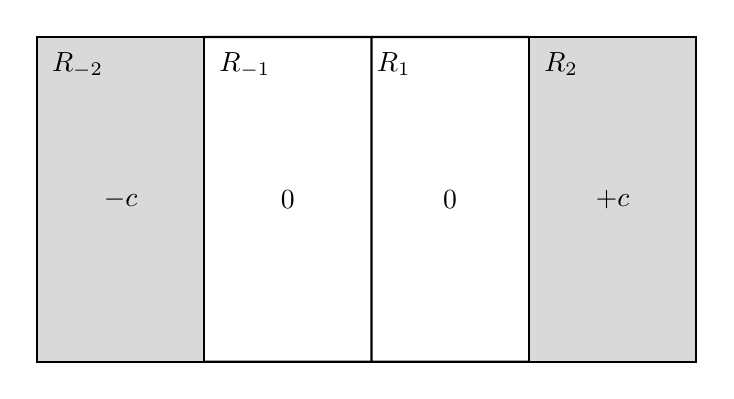
\begin{tikzpicture}[scale=0.8]
\node (A) at (-4,-2) {}; 
\node[right=2 of A.center] (B) {};
\node[right=4 of A.center] (O) {};
\node[right=4 of B.center] (C) {};
\node[right=2 of C.center] (D) {};

\node[above=4 of A.center] (A') {};
\node[above=4 of B.center] (B') {};
\node[above=4 of O.center] (O') {};
\node[above=4 of C.center] (C') {};
\node[above=4 of D.center] (D') {};

\node[right=2 of B.center] (BC) {};
\node[right=2 of B'.center] (B'C') {};

\filldraw[thick, top color=gray!30,bottom color=gray!30] (A.center) rectangle node{$-c$} (B'.center);
\filldraw[thick, top color=gray!30,bottom color=gray!30] (C.center) rectangle node{$+c$} (D'.center);

\node (R1) at ($(B)!0.5!(B'C')$) {0};
\node (R-1) at ($(BC)!0.5!(C')$) {0};

\node [below right = 0.1 of A'.center] {$R_{-2}$};
\node [below right = 0.1 of B'.center] {$R_{-1}$};
\node [below right = 0.1 of O'.center] {$R_{1}$};
\node [below right = 0.1 of C'.center] {$R_{2}$};

\draw[thick] (B.center) -- (C.center);
\draw[thick] (B'.center) -- (C'.center);
\draw[thick] (BC.center) -- (B'C'.center);
\end{tikzpicture}
\end{minipage}
\hfill
\begin{minipage}{0.32\textwidth}
\small
\begin{align*}
R_{-2} &= (-1, -\tfrac{1}{2}) \times (-\tfrac{1}{2}, \tfrac{1}{2}), \\
R_{-1} &= (-\tfrac{1}{2}, 0) \times (-\tfrac{1}{2}, \tfrac{1}{2}), \\
R_{1}  &= (0, \tfrac{1}{2}) \times (-\tfrac{1}{2}, \tfrac{1}{2}), \\
R_{2}  &= (\tfrac{1}{2}, 1) \times (-\tfrac{1}{2}, \tfrac{1}{2}).
\end{align*}
\end{minipage}
\caption{Distribution of rectangles.}
\label{pic:pureinsulation}
\end{figure}
In terms of the functional in \eqref{eye}, the corresponding weight function $f$ is 
\begin{align*}
    f(x) = -c \chi_{R_{-2}} + c \chi_{R_{2}},
\end{align*}
and the central region $R_{-1}\cup R_{1}=(-\frac{1}{2},\frac{1}{2})\times (-\frac{1}{2},\frac{1}{2})$ `insulates' the regions $R_{-2}$ and $R_2$, where $f$ is non-zero, from one another.  Demonstrating \eqref{ins:c} is therefore dubbed the `insulation problem', and it was shown in \cite[Proposition 4.5]{BKV23} that \eqref{ins:c} holds for $c$ in the range $(2,2+\epsilon_0)$ for some $\epsilon_0$.  One of the main results of this paper, Theorem \ref{Thm:insulation}, is that \eqref{ins:c} holds for any $c$ such that $|c|\leq 4$, where the upper bound of $4$ is sharp, and that for $|c|\leq 4$, the unique minimizer of the functional in \eqref{ins:c} is $u=0$.  The technique we use takes advantage of the symmetries of $\om$ and of the functional itself: see Section \ref{insuproper} for the details.  In Theorem \ref{Th:delta} and Proposition \ref{asymptotic}, we consider the effect on $c$ of varying the width of the insulation layer.  The theme of both of these results is that the nonnegativity of the adjusted functional is maintained as long as $|c-2|$ is subordinated to the width of the insulation layer.  The results are not sharp, in contrast to Theorem \ref{Thm:insulation}. 

One can also view the functional in \eqref{eye} as a general form of an `excess functional' associated with an energy $E$ and a suitably-defined stationary point $u_0$, say, so that 
\begin{align}\label{splitting} E(u) = E(u_0)+I(\varphi),\end{align}
with $\varphi=u-u_0$. This is the situation discussed in  \cite{Bevan-14} and \cite{BD22} where, in both cases, the functional $I$ is of the form \eqref{eye}, $f=C\ln(|\cdot|)$, $C$ is constant, and the domain of integration is the unit ball in $\R^2$.  For large enough $C$, \cite[Proposition 3.5 (i)]{Bevan-14} shows that \eqref{meanHad} fails;  by contrast, it can be deduced from \cite[Theorem 1.2]{BD22} that, for sufficiently small $C$, \eqref{meanHad} holds.

 We can take $E=I$ in \eqref{splitting}.  Indeed, if 
 $u=u_0$ on $\Gamma_D\subset \partial \om$ with $u_0\in W^{1,2}(\om; \R^2)$ given then 
 \begin{align}\label{sum}
I(u_0+\varphi)= I(u_0) + \langle I'(u_0),\varphi\rangle +I(\varphi)\ , 
\end{align}
where $I$ is defined in \eqref{eye} and $\varphi\in W^{1,2}(\om;\R^2)$ such that $\varphi=0$ on $\Gamma_D$.  Note that if $u_0$ solves the Euler-Lagrange equations  of  $E$ in the weak sense, i.e., if $\langle E'(u_0),\varphi\rangle=0$  and 
$I(\varphi)\ge 0$ for every $\varphi$ defined above, then $u_0$ is a global  minimizer of $E$. 
This also means that \eqref{sum} implies that for every $\varphi\in W^{1,2}(\om;\R^2)$ such that $\varphi=0$ on $\Gamma_D$ it holds
\begin{align}
    I(u_0+\varphi)\ge I(u_0) + \langle I'(u_0),\varphi\rangle, 
\end{align}
i.e., $I$ is convex.
If we can show that $I(\varphi)=0$ only if $\varphi=0$, then $u_0$ is the unique minimizer of $I$, and $I$ is strictly convex.
%\begin{comment}
%Having established in \cite{BKV23} conditions leading to the mean Hadamard inequality \eqref{eye} in $W_0^{1,n}%%(\om,\R^n)$, it is natural to study the latent convexity    of the functional \eqref{eye} on non-homogeneous classes $W_{u_{0}}^{1,n}(\om,\R^n)$.
%\end{comment}
This idea leads, in the case $n=2$, to a new technique for finding global minimizers of the Dirichlet energy $\D(u)=\int_{\om} |\nabla u|^2 \dx$ in classes where the Jacobian $\det \nabla u$ is \emph{a priori} prescribed pointwise a.e., enabling us to solve the sort of constrained minimization problem %of a type 
that typically arises in incompressible nonlinear elasticity theory (where $g \equiv 1$), but with one important difference.  This is that having first prescribed boundary data $u_0$ and a suitable pressure $f$ in
\begin{align}\label{itwo}I(u):=\int_{\Omega} |\nabla u|^2 + f(x) \,\det \nabla u \, \dx,\end{align}
the data $g$ in the Jacobian constraint emerges (rather than being prescribed \emph{a priori}) as $g:=\det \nabla U$, where $U$ minimizes $I(\cdot)$ in the unconstrained class $W^{1,2}_{u_{0}}(\om,\R^2)$, i.e., the Sobolev space with $u_0$ on $\partial\om$. 

Using this technique, we are able to prove, for example, that for suitable constants $\zeta$ and $\xi$ the map 
\begin{align}\label{examplediskdisk}
    u(x):=\left\{\begin{array}{l l} \zeta x & \ \ x \in B(0,\rho) \\
    \left(\xi+\frac{1-\xi}{|x|^2}\right)x & \ \ x \in B(0,1)\setminus B(0,\rho) \end{array}\right.
    \end{align}
is the unique global minimizer of the Dirichlet energy in 
%\begin{align*}
 $   \left\{v \in W_{\textrm{id}}^{1,2}(B(0,1);\R^2): \ \det \nabla v = g \ \textrm{a.e.}\right\}, $
%\end{align*}
where $g(x):=\zeta^2$ if $x\in B(0,\rho)$ and $g(x):=\xi^2-(1-\xi)^2 |x|^{-4}$ otherwise.  Here, $B(0,\rho)$ stands, as usual, for the ball in $\R^2$ centered at $0$ and of radius $\rho$; see Figure \eqref{problem:disk-disk}. 

\begin{figure}[H]
\centering
\begin{minipage}{1\textwidth}
\centering
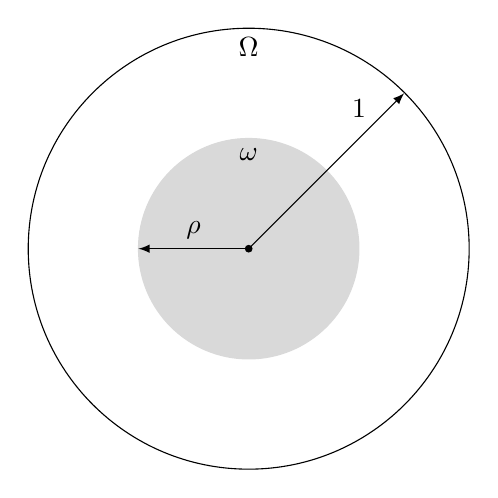
\begin{tikzpicture}[scale=1.4,>=latex]

% Draw disks
\draw (0,0) circle (2.0cm);             % Outer disk (Omega)
\draw[gray!30!,fill] (0,0) circle(1.0cm); % Inner disk (omega)

% Mark center for visual clarity (optional)
\fill (0,0) circle (1pt); % tiny dot at the center

% Labels for domains
\node[below] at (0,1.0) {$\omega$}; 
\node[below] at (0,2.0) {$\Omega$}; 

% Radii arrows from center outward
\draw[->] (0,0) -- (-1.0,0); 
\node[above] at (-0.5,0) {$\rho$}; 

\draw[->] (0,0) -- (1.41,1.41); 
\node[above=4pt] at (1.0,1.0) {$1$}; 

\end{tikzpicture}
\end{minipage}
\caption{Illustration of the disk-disk problem for $\rho = 0.5$.}
\label{problem:disk-disk}
\end{figure}







The relevant weight function or pressure $f=M\chi_{_{B(0,\rho)}}$, where $M$ is a constant such that $|M|<4$.  The functional $I(\varphi)$ is mean coercive in the sense that there exists $\gamma>0$ such that 
\begin{align*}
    I(\varphi) & \geq \gamma \int_{\om}|\nabla \varphi|^2 \, \dx \quad \varphi \in W_0^{1,2}(\om,\R^2),
\end{align*}
which enables us to minimise $I(\cdot)$ in $W_{u_{0}}^{1,2}(B,\R^2)$ and so derive the Euler-Lagrange equation
\begin{align}\label{eltest}
    \int_{B}2\nabla u \cdot \nabla \varphi + M\chi_{_{B(0,\rho)}}\, \cof\nabla u\cdot \nabla\varphi \dx = 0 \quad \quad \varphi \in H^1_0(B,\R^2).
\end{align}

Nevertheless, it is still possible to show that the mean coercivity of $I(\cdot)$ is sufficient to improve the regularity of $W^{1,2}$ solutions of \eqref{eltest} to $C^{0,\alpha}$ for some $\alpha >0$, echoing the results of Morrey \cite[Theorem 4.3.1]{Mo66} and Giaquinta and Giusti \cite{GiaquintaGiusti1982}, for example, and enabling us to `join' pieces of the solution to \eqref{eltest} across the set $\partial B(0,\rho)$ where $f$ is discontinuous, leading in particular to \eqref{examplediskdisk}.  These and related results appeared in \cite{BKV25}.

The paper is organized as follows. In Section~\ref{insuproper}, we introduce and solve the so-called \emph{canonical insulation problem}, which consists of two rectangular regions where $f = c$ and $f = -c$, separated by a subdomain in which $f = 0$. The main result of this section is Theorem~\ref{Thm:insulation}. Proposition~\ref{first-order} further shows that solutions to the Euler--Lagrange equations are minimizers of the associated functional $E_M$ defined in \eqref{EM}. Moreover, uniqueness of the minimizer holds under the additional assumption that $E_M$ is mean coercive.

Section~\ref{thinsulate} addresses configurations in which the intermediate region $f = 0$ between $f = c$ and $f = -c$ is thinner. The main result of this section is Proposition~\ref{asymptotic}.

Finally, Section~\ref{numerics} presents numerical experiments which suggest that the inequalities in Theorem~\ref{Th:delta} and Proposition~\ref{asymptotic} could, in fact, be further strengthened.







\section{The canonical insulation problem}\label{insuproper}

%In this subsection we explore properties of three-state $f$ of the form 
%$$f = \sum_{i=1}^3 M_i\chi_{\om_i},$$
%where $M_i$ are constants and in which each domain $\om_i$ meets at least one other domain $\om_j$ 

We now again focus on the domain 
\begin{equation}\label{domain_insulation}
\Omega := R_{-2} \cup R_{-1} \cup R_1 \cup R_2,
\end{equation}
defined in \eqref{Omega} and shown in Figure~\ref{pic:pureinsulation}.

%To be precise, 
%$$R_1:=[0,\scalebox{0.9}{$\frac{1}{2}$}]\times %[\scalebox{0.9}{$-\frac{1}{2}$},\scalebox{0.9}{$\frac{1}{2}$}]$$
%and 
%$$R_2:=[\scalebox{0.9}{$\frac{1}{2}$},1]\times %[\scalebox{0.9}{$-\frac{1}{2}$},\scalebox{0.9}{$\frac{1}{2}$}]$$
%with $R_{-1}$ and $R_{-2}$ the mirror images of $R_1$ and $R_2$ respectively %in the $x_2$-axis.  
%In the notation introduced above, we therefore have
%\begin{align*}
 %   \om_l  =R_{-2}, \quad
  %  \om_m  =R_{-1}\cup R_1, \quad
   % \om_r  = R_2,
%\end{align*}
%\begin{align*}
%    \om_l & =R_{-2}, \\
%    \om_m & =R_{-1}\cup R_1, \\
%    \om_r & = R_2,
%\end{align*}
%with the middle region $\om_m$ playing the role of an `insulating' layer. 
Let $c>0$ be constant, define the piecewise constant function $f$ by
\begin{align}\label{f_four_square} f(x):=-c\chi_{_{R_{-2}}} + c \chi_{_{R_{2}}}, \end{align}
and form the functional
\begin{align}\label{I_four_square} I\left(\varphi,\INS{-c}{0}{0}{c} \,\right)& := \int_{\om} |\nabla \varphi|^2+f(x) \det \nabla \varphi(x) \dx \\ & = 
\nonumber \int_{\om}|\nabla \varphi|^2 \dx 
- c \int_{R_{-2}} \det \nabla \varphi \dx
+ c\int_{R_2} \det \nabla \varphi \dx 
.
\end{align}


%It is useful to write the functional $I(\varphi,\INS{-c}{0}{0}{c} \,)$ in terms of the odd and even parts of $\varphi$, which we now do.


\begin{theorem}\label{Thm:insulation}
Assume that $|c|\le 4$. Then $I\left(\varphi,\INS{-c}{0}{0}{c} \,\right)\ge 0$ for every $\varphi\in W^{1,2}_0(\Omega;\R^2)$, and the upper bound of $4$ is sharp.
\end{theorem}

\begin{proof}
    Firstly, we may assume that $c\geq 0$, since if this is not the case then we set $\tilde{\varphi}(x_1,x_2)=\varphi(-x_1,x_2)$ and note that 
\begin{align*}
    I\left(\varphi,\INS{-c}{0}{0}{c} \,\right) = I\left(\tilde{\varphi},\INS{c}{0}{0}{-c} \,\right),
\end{align*}
    the point being that it does not matter whether it is $c$ or $-c$ that is attached to the region $R_{-2}$.  Next, we note that it is enough to show the statement for $c=4$.  Indeed, if we assume that $I\left(\varphi,\INS{-4}{0}{0}{4} \,\right) \geq 0$ for all $\varphi$ as above, then by writing
    \begin{align*}
       I\left(\varphi,\INS{-c}{0}{0}{c} \,\right) = \left\{\begin{array}{l l} \int_{\Omega}|\nabla \varphi|^2 \dx + c \Delta \quad &  \quad \mathrm{if}  \ \Delta \geq 0 \\[0.2cm]
       I\left(\varphi,\INS{-4}{0}{0}{4} \,\right) + (c-4)\Delta  \quad & \quad \mathrm{if} \ \Delta < 0,
       \end{array}\right.
    \end{align*}
where $$\Delta: = \int_{R_{2}}\det \nabla \varphi \, \dx - \int_{R_{-2}}\det \nabla \varphi \, \dx,$$
it is clear that $I\left(\varphi,\INS{-c}{0}{0}{c} \,\right) \geq 0$ for the same $\varphi$ and $0 \leq c \leq 4$.  Henceforth, we set $I(\varphi):=I\left(\varphi,\INS{-4}{0}{0}{4} \,\right)$ for brevity.
%    because if $I$ is negative for some $\varphi$  then $\int_{R_{-2}}\det\nabla\varphi(x)\, \dx>0$ or  $\int_{R_{2}}\det\nabla\varphi(x)\, \dx<0$ so that taking $|c|$ larger makes the value of the functional $I$ smaller. 
Moreover, it is easy to see that in order to minimise $I(\varphi)$ we can assume that 
    $\varphi$ is symmetric with respect to the line $x_1=0$, i.e., $\varphi(x_1,x_2)=\varphi(-x_1,x_2)$ for all $x_1\in [0,1]$.
\begin{comment}
Now consider the decomposition $I(\varphi) = I^-(\varphi) + I^+(\varphi)$, where
\begin{align*}
   I(\varphi)= \underbrace{\int_{R_{-2}} |\nabla \varphi|^2 - 4 \det \nabla \varphi \dx + \int_{R_{-1}} |\nabla\varphi|^2 \, \dx}_{=:I^-(\varphi)} + \underbrace{\int_{R_2} |\nabla \varphi|^2 + 4 \det \nabla \varphi \dx + \int_{R_1} |\nabla\varphi|^2 \, \dx}_{=:I^+(\varphi)}.
\end{align*}
If it holds that $I^+(\varphi) \leq I^-(\varphi)$, then by reflecting $\varphi$ in the line $x_1=0$ using $\tilde{\varphi}$ defined above, we have
$I^{+}(\varphi) = I^{-}(\tilde{\varphi})$.  Otherwise, $I^+(\varphi) \geq I^-(\varphi)$, 
\end{comment}
Hence, it suffices to show that     
\begin{align}\label{half-domain}
   E(u)= \int_{R_{-2}} |\nabla u|^2 -4 \det\nabla u\,\dx +\int_{R_{-1}}|\nabla u |^2\,\dx\ge 0 
\end{align}    
for any $u\in W^{1,2}(\om;\R^2)$ such that $u=0$ on  $\partial(R_{-2}\cup R_{-1})\setminus\{x_1=0\}$, see Figure \ref{pic:pureinsulation_reduced}.
\begin{figure}[H]
\centering
\begin{minipage}{0.69\textwidth}
\centering
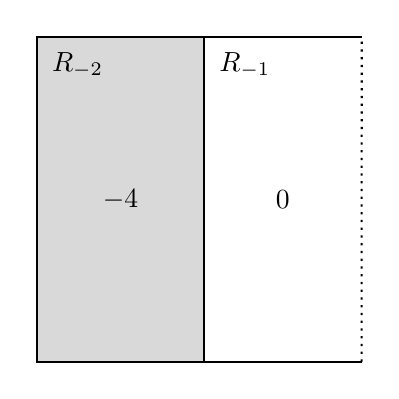
\begin{tikzpicture}[scale=0.8]
% Define main points
\node (A) at (-4,-2) {}; % bottom-left corner of R_{-2}
\node[right=2 of A.center] (B) {}; % interface between R_{-2} and R_{-1}
\node[right=4 of A.center] (O) {}; % right edge (x=0)

% Top corners (4 units above)
\node[above=4 of A.center] (A') {};
\node[above=4 of B.center] (B') {};
\node[above=4 of O.center] (O') {};

% Shaded rectangle over R_{-2}
\filldraw[thick, top color=gray!30, bottom color=gray!30] (A.center) rectangle node{$-4$} (B'.center);

% Label 0 in R_{-1}
\node at ($(B)!0.5!(O')$) {0};

% Region labels
\node[below right=0.1 of A'.center] {$R_{-2}$};
\node[below right=0.1 of B'.center] {$R_{-1}$};

% Vertical boundaries
\draw[thick] (B.center) -- (O.center);
\draw[thick] (B'.center) -- (O'.center);

% Free boundary at x=0 (dotted)
\draw[thick, dotted] (O.center) -- (O'.center);

% Optional coordinate labels (uncomment if desired)
% \node[below] at (A) {$x=-4$};
% \node[below] at (B) {$x=-2$};
% \node[below] at (O) {$x=0$};
\end{tikzpicture}
\end{minipage}
\caption{Part of the domain $\Omega$ divided into rectangles \( R_{-2} \) and \( R_{-1} \); boundary conditions of \(u\): solid lines = zero value, dotted line = free boundary.}
\label{pic:pureinsulation_reduced}
\end{figure}

Condition \eqref{half-domain} is equivalent to 
$$
J(u,\psi):= \int_{R_{-2}} |\nabla u|^2 -4 \det\nabla u +|\nabla u+\nabla\psi|^2\,\dx \ge 0 $$

for all $u$ as above and all $\psi\in W^{1,2}(\om;\R^2)$ such that  $\psi=0$ on  $\partial(R_{-2}\cup R_{-1})\setminus\{x_1=-1\}$.

Given $u$ and $\psi $ we construct $\varphi$ as follows:

$$
\varphi(x):=
\begin{cases}
    u(x)  & \text{ if } x\in R_{-2},\\
 u(-x_1-1,x_2)+\psi(-x_1-1,x_2)    & \text{ if } x\in R_{-1},\\
 \varphi(-x_1,x_2) & \text{ if } x\in R_{1}\cup R_2,\end{cases}
$$
from which it follows that $E(\varphi)= J(u,\psi)$.  Keeping in mind that $|\cof A|=|A|$  and $2\det A=\cof A:A$ for any $A\in\R^{2\times 2}$,
we calculate
\begin{align*}
J(u,\psi)&= \int_{R_{-2}} |\cof\nabla u|^2 -4 \det\nabla u +|\nabla u|^2+|\nabla\psi|^2 + 2\nabla u:\nabla\psi\,\dx\\
&=\int_{R_{-2}} |\cof\nabla u-\nabla u|^2 +|\nabla\psi|^2 + 2\nabla u:\nabla\psi\,\dx\\
&= \int_{R_{-2}}|(\cof\nabla u-\nabla u)-\nabla\psi|^2+2(\cof\nabla u-\nabla u):\nabla \psi+2\nabla u:\nabla\psi\,\dx\\
&=\int_{R_{-2}}|\cof\nabla u-\nabla u-\nabla\psi|^2\,\dx\ge 0,
\end{align*}
where we have applied Lemma~\ref{Jon'slemma} below.  Finally, if $c>4$ (or, equivalently, $c<-4$), we can apply \cite[Proposition 3.4]{BKV23} in order to find $\varphi_0 \in W^{1,2}(\om,\R^2)$ such that $I(\varphi_0)<0$, so that the upper bound of $4$ in $|c|\leq 4$ is sharp.
\end{proof}

\begin{lemma}\label{Jon'slemma}
 It holds that $$\int_{R_{-2}}\cof\nabla u:\nabla\psi\,\dx=\int_{R_{-2}}\cof\nabla\psi :\nabla u\dx =0$$   for all $u$ and $\psi$ as in the proof of Theorem~\ref{Thm:insulation}.
\end{lemma}

\begin{proof}
    We get in view of the Piola identity ${\rm div}\,\,\cof\nabla u= {\rm div}\,\,\cof\nabla \psi=0$ that 
    $$
    \int_{R_{-2}}\cof\nabla u:\nabla\psi\,\dx=\int_{\partial R_{-2}} (\cof\nabla u)\nu\cdot\psi\,{\rm d}S=\int_{\partial R_{-2}} (\cof\nabla \psi)\nu\cdot u\,{\rm d}S , $$
    where $\nu$ is the unit outer normal to the boundary of $R_{-2}$.
    Note that $\psi=0$ on three faces of $R_{-2}$, and, on the face $x_1=-1$,  $u=0$, which implies that $(\cof\nabla u)\nu$  is zero along the boundary as well. 
    The statement follows. 
    \end{proof}









\begin{corollary}
If $J(u,\psi)=0$ if and only if $u=\psi=0$ in $R_{-2}$.
\end{corollary}
\begin{proof}
The "if" implication is trivial. We focus on the opposite one.
By Theorem 1, $J(u,\psi)=0$ only if 
\begin{align}\label{Martin'sidentity}\cof \, \nabla u - \nabla u = \nabla \psi \quad \mathrm{a.e. \ in} \ R_{-2}.
\end{align}
Taking the inner product of this expression with $\cof \, \nabla u$ and integrating over $R_{-2}$ gives 
\begin{align}\label{conformal}\int_{R_{-2}}|\nabla u|^2 - 2 \det \nabla u \, \dx = 0,
\end{align}
where we have again made use of Lemma \ref{Jon'slemma}. By Hadamard's pointwise inequality for matrices in $\R^{2 \times 2}$, \eqref{conformal} implies that for a.e.\@ $x$ in $R_{-2}$ $\cof \nabla u(x) = \nabla u(x)$, i.e. $\nabla u(x)$ is conformal.  Using this and \eqref{Martin'sidentity}, it follows that $\nabla \psi=0$ a.e.\@ in $R_{-2}$, and hence, by the boundary conditions, $\psi=0$.  Moreover, since $\nabla u$ is conformal then the function $f: z=x+iy \mapsto u_1(x,y)+iu_2(x,y)$ is holomorphic in $R_{-2}$.  Let $a$ be the midpoint of the line joining $-1-i/2$ and $-1/2-i/2$, and note that the function
\begin{align*}
    \widetilde{f}(z)& :=\left\{ \begin{array}{l l } f(z) & \mathrm{if} \ \im z \geq -1/2  \\
    \overline{f(\bar{z}-i)} & \mathrm{if} \ \im z \leq -1/2 
    \end{array}\right.
\end{align*}
is, by applying the boundary condition $f(z)=0$ for $z \in R_{-2}$ such that $\im z = -1/2$ together with the Schwarz reflection principle, holomorphic in a sufficiently small disk $D(a,r)$ about the point $a$.  The set $\{z\in D(a,r): \ \widetilde{f}(z)=0\}$ clearly contains an accumulation point, so by standard results it holds that $\widetilde{f}(z) = 0$ for $z$ in $D(a,r)$, and in particular that $f(z)=0$ for  $z$ in $D(a,r) \cap R_{-2}$.  It now follows that $f=0$ in $R_{-2}$, so $u=0$ there. 


\end{proof}

\begin{remark}\label{BC}
    It follows from the proof of Lemma~\ref{Jon'slemma} that the statement of the lemma holds true if 
    on the boundary $u=0$ or $\psi=0$. Hence, $J(u,\psi)\ge 0$ in much more general situations. For instance,  we need only to assume that $\psi=0$ on the part of the boundary where $x_1=-1/2$.
\end{remark}
    
\subsection{Uniqueness of minimizers for polyconvex integrands}
    Let us put $R=R_{-2}\cup R_{-1}$. Consequently,  it follows for $E$ given in \eqref{half-domain} that  $E(u)\ge 0$ if $u\in W^{1,2}(R;\R^2)$  such that $u=0$  on $\partial R_2\setminus\{x:\, x_1=-1/2\}$.
Let us define for $u\in W^{1,2}(R;\R^2)$ and $M\in\R$
\begin{align}\label{EM}
    E_M(u)= \int_{R_{-2}} |\nabla u|^2 -M \det\nabla u\,\dx +\int_{R_{-1}}|\nabla u |^2\,\dx \end{align}


\begin{proposition}\label{first-order}
    Let $0\le M<4$ then 
    $$E_M(u)\ge \frac{4-M}{4}\int_{R} |\nabla u|^2\,\md x$$ for every $u\in W^{1,2}(R;\R^2)$  such that $u=0$  on $\partial R_2\setminus\{x:\, x_1=-1/2\}$, i.e., $E_M$ is mean coercive. 
    \end{proposition}

    \begin{proof}
        In view of Remark~\ref{BC} and the fact that $E_4=E$ given in \eqref{half-domain} we have that $E_4\ge 0$. 
        Finally, 
        $$E_4(u)=\frac4M E_M(u)-(4/M-1)\int_{R} |\nabla u|^2\,\md x\ge 0 $$
        and the result follows.
    \end{proof}

Consider $u_0\in W^{1,2}(R;\R^2)$ and define 
$$\mathcal{U}_{u_0} =\{u\in W^{1,2}(R;\R^2):\,  \textrm{ such that } u=u_0  \textrm{ on } \partial R_2\setminus\{x:\, x_1=-1/2\} \}. $$

If $\psi\in \mathcal{U}_{u_0}$ and $u\in \mathcal{U}_0$ then 
\begin{align}\label{minimizer}
E_M(\psi+ u)=E_M(\psi)+\langle E'(\psi),u\rangle +E_M(u)\ .
\end{align}

The next proposition shows that solutions of the Euler-Lagrange equations for $E_M$  with mixed boundary conditions are minimizers of $E_M$ despite the fact that the integrand is not convex.  This is an analogous result to \cite{neff}, see also \cite{john,spector,spector2} for uniqueness results in nonlinear elasticity. 

\begin{proposition}
    Let $0<M\le 4$ and let  $\psi\in\mathcal{U}_{u_0}$ be such that  $\langle E'(\psi),u\rangle=0$. Then $\psi$ is a minimizer 
    of $E_M$ on $\mathcal{U}_{u_0}$  which is unique for $M<4$.
\end{proposition}

\begin{proof}
It follows from \eqref{minimizer} and from mean coercivity of $E_M$ for $0\le M<4$.
\end{proof}

\subsection{Varying the width of the insulation layer}\label{thinsulate}

In this section we consider the effect of varying the width of the so-called insulation layer, which in Section \ref{insuproper} corresponded to the region $R_{-1} \cup R_{1}$ and which was of unit width. The intuition is that the thinner the insulation region, the smaller the range of $c$ for which the corresponding excess function is nonnnegative. 

Evidence for this is supplied by Theorem \ref{Th:delta} and Proposition \ref{asymptotic} below, a consequence of which is the result that if $N \in\N$ and the canonical domain is replaced with
$$\Omega_{N}:=\left(-\frac{1}{2}-\frac{1}{2N},\frac{1}{2}+\frac{1}{2N}\right) \times \left(-\frac{1}{2}, \frac{1}{2}\right),$$
consisting of the regions 
\begin{align*}R_{-2,N} & =\left(-\frac{1}{2}-\frac{1}{2N},-\frac{1}{2N}\right) \times \left(-\frac{1}{2},\frac{1}{2}\right) \ \mathrm{and} \\
R_{2,N} & =\left(\frac{1}{2N},\frac{1}{2}+\frac{1}{2N}\right) \times \left(-\frac{1}{2},\frac{1}{2}\right)\end{align*} which are separated by a `thin' insulation layer $\left(-\frac{1}{2N},\frac{1}{2N}\right) \times \left(-\frac{1}{2},\frac{1}{2}\right)$, and if 
$$f(x):= c \chi_{R_{2,N}} - c \chi_{R_{-2,N}},$$
then for all $\varphi \in W_0^{1,2}(\om_N,\R^2)$ we have
\begin{align}\label{inequalityN} \int_{\om_N} |\nabla u|^2 + f(x) \det \nabla u \, \dx \geq 0 \quad \mathrm{if}  |c| \lesssim 2 + \frac{2}{N}.\end{align} 
As the insulation region shrinks, we see that the upper bound in the sufficient condition $|c| \lesssim 2 + \frac{2}{N}$ approaches 2.  The extent to which this is necessary is investigated numerically in Section \ref{theorem5numerics} and, at least for reasonable values of $N$, there is evidence that the upper bound $2 + \frac{2}{N}$ is far from necessary other than in the case $N=1$, but with a similar (decreasing) trend.   

Using the symmetry of the domain $\om_N$, we can argue as we did for the canonical insulation problem that in order to prove \eqref{inequalityN} it is sufficient to show 
$$\int_{R_{-2,N}}|\nabla u|^2 - c \det \nabla u \, \dx + \int_{(-1/2N,0)\times (-1/2,1/2)} |\nabla u|^2 \geq 0$$
for all $u$ in $W^{1,2}(R_{-2,N}\cup (-1/2N,0)\times (-1/2,1/2);\R^2)$ such that $u=0$ on the boundary of that region other than along $\{0\} \times (-1/2,1/2)$.  Then, by a translation of $-\frac{1}{2}$ along the $x_1$ axis, we further argue that it is sufficient to prove 
$$\int_{R_{-2}}|\nabla u|^2 - c \det \nabla u \, \dx + \int_{R^\delta} |\nabla u|^2 \, \dx \geq 0$$
for all $u$ in $W^{1,2}(R_{-2} \cup R^\delta;\R^2)$ such that $u=0$ on $\partial(R_{-2}\cup R^{\delta})\setminus \{x:\, x_1=-1/2+\delta\}$. Here, $R^\delta=(-1/2,-1/2+\delta)\times(-1/2,1/2)$ and $R_{-2}$ is defined in Figure \ref{pic:pureinsulation}. 





To that end, it follows from \cite{BKV23,mielke-sprenger} that $\forall\varepsilon>0$  there exists $u_\varepsilon\in W^{1,2}(R_{-2};\R^2)$, $u_\varepsilon=0$ on $\partial R_{-2}\setminus \{x_1=-1/2\}$ such that 
\begin{align}\label{ms}
    \int_{R_{-2}}|\nabla u_\varepsilon|^2 \,\md x < (2+\varepsilon)\int_{R_{-2}}\det\nabla u_\varepsilon\,\md x\ .
\end{align}
Let us denote the set of such maps $\mathcal{A}_\varepsilon$, i.e.,
$$\mathcal{A}_\varepsilon=\{u_\varepsilon\in W^{1,2}(R_{-2};\R^2):\, u_\varepsilon=0 \text{ on }\partial R_{-2}\setminus \{x_1=-1/2\}, \text{ and  \eqref{ms} holds }\}\ .$$
Hence, given $2<M<4$ we get for $\varepsilon>0 $ small enough
 \begin{align}\label{lower-upper bound}
   \frac{2-M}{2}\int_{R_{-2}}|\nabla u_\varepsilon|^2 \,\md x&\le \int_{R_{-2}}|\nabla u_\varepsilon|^2 \,\md x -M\int_{R_{-2}}\det\nabla u_\varepsilon\,\md x\nonumber\\\
&    <\int_{R_{-2}}|\nabla u_\varepsilon|^2 \,\md x -\frac{M}{2+\varepsilon} \int_{R_{-2}}|\nabla u_\varepsilon|^2 \,\md x\nonumber\\\
   &= \frac{2+\varepsilon-M}{2+\varepsilon} \int_{R_{-2}}|\nabla u_\varepsilon|^2 \,\md x\nonumber\\
   &<\frac{2+\varepsilon-M}{2} \int_{R_{-2}}|\nabla u_\varepsilon|^2 \,\md x.
\end{align} 

Let us extend $u_\varepsilon$ to the domain $$R^\delta=(-1/2,-1/2+\delta)\times(-1/2,1/2), \quad \text{where } \delta=(M-2)/4 $$ such that this extension has zero Dirichlet boundary conditions on the set $\{x_2=\pm 1/2\}$, see Figure  \ref{pic:pureinsulation_reduced_general}.

\begin{figure}[H]
\centering
\begin{minipage}{0.69\textwidth}
\centering
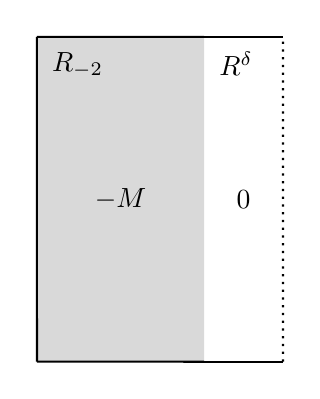
\begin{tikzpicture}[scale=0.8]
% Define main points
\node (A) at (-4,-2) {}; % bottom-left corner of R_{-2}
\node[right=2 of A.center] (B) {}; % interface between R_{-2} and R_{-1}
\node[right=3 of A.center] (O) {}; % right edge (x=0)

% Top corners (4 units above)
\node[above=4 of A.center] (A') {};
\node[above=4 of B.center] (B') {};
\node[above=4 of O.center] (O') {};

% Shaded rectangle over R_{-2}
\fill[thick, top color=gray!30, bottom color=gray!30] (A.center) rectangle node{$-M$} (B'.center);
% Left boundary
\draw[thick] (A.center) -- (A'.center);

% Bottom boundary
\draw[thick] (A.center) -- (B.center);

% Top boundary
\draw[thick] (A'.center) -- (B'.center);

% Label 0 in R_{-1}
\node at ($(B)!0.5!(O')$) {0};

% Region labels
\node[below right=0.1 of A'.center] {$R_{-2}$};
\node[below right=0.1 of B'.center] {$R^{\delta}$};

% Vertical boundaries
\draw[thick] (B.center) -- (O.center);
\draw[thick] (B'.center) -- (O'.center);

% Free boundary at x=0 (dotted)
\draw[thick, dotted] (O.center) -- (O'.center);

% Optional coordinate labels (uncomment if desired)
% \node[below] at (A) {$x=-4$};
% \node[below] at (B) {$x=-2$};
% \node[below] at (O) {$x=0$};
\end{tikzpicture}
\end{minipage}
\caption{Part of the domain $\Omega$ divided into rectangles \( R_{-2} \) and \( R^{\delta} \); 
boundary conditions for \(u\): solid lines indicate zero value, the dotted line indicates a free boundary. 
Note that the horizontal lengths of \( R_{-2} \) and \( R^{\delta} \) are \(1/2\) and 
\(\delta = (M-2)/4\), respectively.}
\label{pic:pureinsulation_reduced_general}
\end{figure}











\begin{lemma}\label{lowerbound}
 If $2<M\le 3$, $2/(M-2)\in \mathbb{N}$ and $\delta=(M-2)/4$
 then 
\begin{align}\label{special}
  \int_{R^\delta}|\nabla u_\varepsilon|^2 \,\md x  \ge \frac{M-2-\varepsilon}{2} \int_{R_{-2}}|\nabla u_\varepsilon|^2 \,\md x\ .
\end{align} 
 
for every $u_\varepsilon\in\mathcal{A}_\varepsilon$ defined above and 
every $0<\varepsilon<M-2$.
    
\end{lemma}

\begin{proof}
    
Assume that 
\begin{align}
  \int_{R^\delta}|\nabla u_\varepsilon|^2 \,\md x  < \frac{M-2-\varepsilon}{2} \int_{R_{-2}}|\nabla u_\varepsilon|^2 \,\md x\ .
\end{align}
This implies that 
\begin{align}
   \int_{R_{-2}}|\nabla u_\varepsilon|^2 \,\md x -M\int_{R_{-2}}\det\nabla u_\varepsilon\,\md x+ \int_{R^\delta}|\nabla u_\varepsilon|^2 \,\md x<0\ .
\end{align}

Let us further assume that $2/(M-2)\in\mathbb{N}$.
 We extend $u_\varepsilon$ from $R^\delta$ to $R_{-1}$ by 2/(M-2)  flips along the vertical direction   so that 
 \begin{align}\label{upper-bound}
     \int_{R_{-1}}|\nabla u_\varepsilon|^2 \,\md x=\frac{2}{M-2} \int_{R^\delta}|\nabla u_\varepsilon|^2 \,\md x<
     \frac{(M-2-\varepsilon)}{(M-2)}\int_{R_{-2}}|\nabla u_\varepsilon|^2 \,\md x
 \end{align}

 We have 
 \begin{align}\label{M=4}
    \int_{R_{-2}}|\nabla u_\varepsilon|^2 -4\int_{R_{-2}}\det\nabla u_\varepsilon\,\md x <  \int_{R_{-2}}|\nabla u_\varepsilon|^2 -\frac{4}{2+\varepsilon} \int_{R_{-2}}|\nabla u_\varepsilon|^2\, \md x=\frac{\varepsilon-2}{\varepsilon+2}\int_{R_{-2}}|\nabla u_\varepsilon|^2\, \md x\ .
 \end{align}

 Putting together \eqref{M=4} and \eqref{upper-bound}
we get for $2<M\le 3$
\begin{align}
  \int_{R_{-2}}|\nabla u_\varepsilon|^2 -4\int_{R_{-2}}\det\nabla u_\varepsilon\,\md x+ \int_{R_{-1}}|\nabla u_\varepsilon|^2 \,\md x< \frac{\varepsilon\,(2M-6-\varepsilon)}{(\varepsilon+2)(M-2)}\int_{R_{-2}}|\nabla u_\varepsilon|^2\, \md x <0\ ,
\end{align}
 which contradicts Theorem~\ref{Thm:insulation} whenever $2<M\le 3$. 

 \end{proof}
Hence, adding \eqref{upper-bound} to both sides of \eqref{lower-upper bound} yields 
\begin{align*}
   \frac{-\varepsilon}{2}\int_{R_{-2}}|\nabla u_\varepsilon|^2 \,\md x&\le \int_{R_{-2}}|\nabla u_\varepsilon|^2 \,\md x -M\int_{R_{-2}}\det\nabla u_\varepsilon\,\md x+\int_{R^\delta}|\nabla u_\varepsilon|^2 \,\md x \\
\end{align*} 

and therefore 
\begin{align}\label{epsilon}
   0\le  \int_{R_{-2}}\frac{2+\varepsilon}{2}|\nabla u_\varepsilon|^2 \,\md x -M\int_{R_{-2}}\det\nabla u_\varepsilon\,\md x+\int_{R^\delta}|\nabla u_\varepsilon|^2 \,\md x 
\end{align} 
whenever $u_\varepsilon\in\mathcal{A}_\varepsilon.$

\begin{theorem} \label{Th:delta}
    Let $2\le M\le 3$ such that $2/(M-2)\in\mathbb{N}$ for $M>2$. Let further $\delta=(M-2)/4$  Then 
    \begin{align}\label{thm2-ineq}
   \frac{\int_{R_{-2}}|\nabla u|^2 \,\md x}{2\int_{R_{-2}}\det\nabla u\,\md x} \int_{R_{-2}}|\nabla u|^2 \,\md x-M\int_{R_{-2}}\det\nabla u\,\md x+ \int_{R^\delta}|\nabla u|^2 \,\md x\ge 0\ 
\end{align}
for every $u\in W^{1,2}(R_{-2}\cup R^\delta;\R^2)$, $u=0$ on $\partial ( R_{-2}\cup R^\delta)\setminus \{x:\, x_1=-1/2+\delta\}$ such that $\int_{R_{-2}}\det\nabla u\,\md x>0$. %In particular, if $M=3$ then $\delta =1/4$.
\end{theorem}

\begin{proof} If $M=2$ then $\delta=0$ and the statement follows from the pointwise Hadamard inequality.
    Assume that $M>2$ and that the statement is not true, i.e., that there is $u$ admissible such that  \eqref{thm2-ineq} does not hold. 
    Then inevitably 
\begin{align}
   \int_{R_{-2}}|\nabla u|^2 \,\md x -M\int_{R_{-2}}\det\nabla u\,\md x<0\ .
   \end{align}
   This means that there is $2+\varepsilon<M$ such that 
\begin{align}
   \frac{M}{2+\varepsilon}\int_{R_{-2}}|\nabla u|^2 \,\md x -M\int_{R_{-2}}\det\nabla u\,\md x<0\ .
   \end{align}   
 However, then $u\in\mathcal{A}_\varepsilon$ where $2+\varepsilon > \int_{R_{-2}}|\nabla u|^2 \,\md x /\int_{R_{-2}}\det\nabla u\,\md x$. Consequently, \eqref{epsilon} holds for this $u$ and $\varepsilon$ instead of $u_\varepsilon$. 
 Taking the infimum over $\varepsilon$ gives the result.
    
\end{proof}

\begin{remark}\label{expansion_delta}
We believe that the factor $\int_{R_{-2}}|\nabla u|^2 \,\md x /(2\int_{R_{-2}}\det\nabla u\,\md x)\ge 1$ in Theorem~\ref{Th:delta} can be omitted, and the numerical tests below confirm it.  The admissible pairs of Theorem~\ref{Th:delta} are exactly
\[
(\delta, M)=\Bigl(\tfrac{1}{2k},\,2+\tfrac{2}{k}\Bigr), \qquad k\in\mathbb{N}.
\]
For $k=1$, one obtains the setup of Theorem~\ref{Thm:insulation}. 
\end{remark}
In the spirit of Theorem \ref{Th:delta}, we have the following result.  
\begin{proposition}\label{asymptotic}
Let $k \in \N$ and set
\begin{align}\label{mk}M_k:=1-\frac{1}{k}+\left(\frac{1}{k^2}+\frac{6}{k}+1\right)^{\frac{1}{2}}\end{align}
and set $\delta:=\frac{1}{2k}$.  Then for every $u\in W^{1,2}(R_{-2}\cup R^\delta;\R^2)$ such that $u=0$ on $\partial ( R_{-2}\cup R^\delta)\setminus \{x_1=-1/2+\delta\}$, it holds that 
\begin{align}\label{marmite}
\int_{R_{-2}}|\nabla u|^2 - M_k \det \nabla u \dx + \int_{R^{\delta}}|\nabla u|^2 \,\dx \geq 0.
\end{align}
\end{proposition}
\begin{proof}
    Assume for a contradiction that \eqref{marmite} is false for one of the $u$ in the class described.  Then $u$ is not zero and
    \begin{align}
   \label{firstline}    \int_{R^{\delta}} |\nabla u|^2 \, \dx & < \int_{R_{-2}} M_k \det \nabla u - |\nabla u|^2 \, \dx \\ \nonumber
       & \leq \int_{R_{-2}} M_k \det \nabla u - 2 |\det \nabla u| \, \dx \\ \nonumber
       & \leq  (M_k-2)\int_{R_{-2}} |\det \nabla u| \, \dx \\
\label{marmalade}     \int_{R^{\delta}} |\nabla u|^2 \, \dx  & \leq   \frac{M_k-2}{2}\int_{R_{-2}} |\nabla u|^2 \, \dx,
    \end{align}
where we have used Hadamard's pointwise inequality $|\nabla u|^2 \geq 2 |\det \nabla u|$ twice.  Now extend $u$ to a function $\tilde{u}$ in $W^{1,2}(R_{-2} \cup R_{-1})$ by a sequence of $k-1$ reflections of $u\arrowvert_{_{R^{\delta}}}$ in vertical lines that cross the $x_1-$axis at points $-1/2+n \delta$ for $n=1,\ldots,k-1$, and note that by \eqref{marmalade} and because $\tilde{u}=u$ on $R_{-2}$, we have
\begin{align}\label{jam}\int_{R_{-1}}|\nabla \tilde{u}|^2 \, \dx < \frac{k(M_k-2)}{2}\int_{R_{-2}} |\nabla \tilde{u}|^2 \, \dx. 
\end{align}

Note also that by rearranging \eqref{firstline} it follows that 
\begin{align}
    \label{lemoncurd} \int_{R_{-2}}\det \nabla \tilde{u} \, \dx > \frac{1}{M_k} \int_{R_{-2}} |\nabla \tilde{u}|^2 \, \dx. 
\end{align}

Now consider the quantity
$$I(\tilde{u})=\int_{R_2}|\nabla \tilde{u}|^2 - 4\det \nabla \tilde{u} \, \dx + \int_{R_{-1}} |\nabla \tilde{u}|^2 \, \dx,$$ 
and note that by \eqref{jam} and \eqref{lemoncurd}
\begin{align*}
  I(\tilde{u}) & \leq \int_{R_{-2}} |\nabla \tilde{u}|^2 -\frac{4}{M_k}|\nabla \tilde{u}|^2 + \frac{k(M_k-2)}{2} |\nabla \tilde{u}|^2 \, \dx \\
  & = \left( 1 -\frac{4}{M_k} + \frac{k(M_k-2)}{2} \right)\int_{R_{-2}}|\nabla \tilde{u}|^2 \, \dx. 
\end{align*}
But $M_k$ given by \eqref{mk} is such that 
$$  1 -\frac{4}{M_k} + \frac{k(M_k-2)}{2} = 0,$$
which implies $I(\tilde{u})=0$.  By Theorem~\ref{Thm:insulation}, this is possible only if $\tilde{u}$ is zero, which is contrary to our initial assumption. 
\end{proof}

We remark that for large $k$ the constants $M_k$ given by \eqref{mk} obey
$$M_k \sim 2 + \frac{2}{k} - \frac{1}{2k^2} + o\left(\frac{1}{k^2}\right),$$
so that we recover, albeit asymptotically, the result of Theorem \ref{Th:delta}, and without the need for additional hypotheses. 

\section{Numerical experiments}\label{numerics}

The functional \eqref{I_four_square} reads
\begin{equation}\label{I_four_square_fem}
I(\varphi)
=
\int_{\Omega}
\nabla \varphi : \nabla \varphi
+
\frac12\, f \, \nabla \varphi : \operatorname{cof}\nabla \varphi
\,\mathrm{d}x,
\end{equation}
where \( : \) denotes the Frobenius inner product on \( \mathbb{R}^{2\times2} \).
Using the identity \( A:\operatorname{cof}A = 2\det A \), the second term can be interpreted as a determinant contribution.

Let \( V_h \subset W^{1,2}(\Omega;\mathbb{R}^2) \) be a finite element space of continuous, piecewise affine vector fields over a triangular mesh aligned with the jump set of \(f\); see Figure~\ref{mesh}.

\begin{figure}[htbp]
    \centering
    \includegraphics[width=0.99\textwidth]{mesh_and_f.png}
    \caption{Example of a level 3 triangular mesh of \( \Omega \) (left) and the distribution of \( f \) (right).}
    \label{mesh}
\end{figure}

\noindent
The approximation \( \varphi_h \in V_h \) is represented as
\[
\varphi_h = \sum_{i=1}^N v_i \phi_i,
\qquad
\mathbf v=(v_1,\dots,v_N)^\top\in\mathbb{R}^N,
\]
where \( \{\phi_i\}_{i=1}^N \) is the standard finite element basis of globally continuous, piecewise affine vector-valued functions associated with the mesh nodes. These basis functions satisfy the nodal interpolation property \( \phi_i(x_j)=\delta_{ij} \), so that the coefficient vector \( \mathbf v \) represents the nodal values of the discrete deformation:
\[
\varphi_h(x_i) = v_i.
\]

Since the basis functions are affine on each triangle, their gradients are piecewise constant, and thus
\[
\nabla \varphi_h = \sum_{i=1}^N v_i \nabla \phi_i.
\]

Substituting this expansion into \eqref{I_four_square_fem} and exploiting bilinearity, we define the stiffness matrices (cf.~\cite{BKV25})
\[
(K_1)_{ij}
=
\int_{\Omega} \nabla \phi_j : \nabla \phi_i\,\mathrm{d}x,
\qquad
(K_2)_{ij}
=
\int_{\Omega}
f\, \nabla \phi_j : \operatorname{cof}\nabla \phi_i\,\mathrm{d}x,
\]
which leads to the quadratic representation
\begin{equation}\label{quadratic_form}
I(\varphi_h)
=
\mathbf v^{\top}
\bigl(K_1+\tfrac12 K_2\bigr)\,
\mathbf v
=:
\mathbf v^{\top}
A \,
\mathbf v.
\end{equation}

\noindent
The matrix \( A \) is symmetric. The positivity of its minimal eigenvalue \( \lambda_{\min}(A) \) guarantees that the quadratic form \eqref{quadratic_form} is positive definite and hence confirms Theorem~\ref{Thm:insulation}, while \( \lambda_{\min}(A) < 0 \) indicates a violation.

Equivalently, positive definiteness of \( A \) can be verified by the existence of a Cholesky factorization \( A = LL^\top \). In the computations, failure of the Cholesky decomposition provides a practical indicator of the loss of positive definiteness.

\begin{comment}
\subsection{Numerical verification}
For \( n = 2 \), the functional \eqref{I_four_square} can be written as
\begin{align}\label{I_four_square_fem}
I(\varphi)
:=
\int_{\Omega}
\nabla \varphi : \nabla \varphi
+ \frac{1}{2}\, f \, \nabla \varphi : \operatorname{cof} \nabla \varphi
\, \mathrm{d}x,
\end{align}
where \( : \) denotes the Frobenius inner product on \( \mathbb{R}^{2\times2} \).
Using the identity \( A : \operatorname{cof} A = 2 \det A \) for all \( A \in \mathbb{R}^{2\times2} \), the cofactor term may be equivalently expressed as a determinant.

The finite element approximation \( \varphi_h \in V_h \) is expressed as a linear combination of vector-valued basis functions \( \{\phi_i\}_{i=1}^N \), where each \( \phi_i : \Omega \to \mathbb{R}^2 \) belongs to the finite-dimensional subspace \( V_h \subset W^{1,2}(\Omega;\mathbb{R}^2) \):
\begin{equation*}
\varphi_h(x) = \sum_{i=1}^N v_i \, \phi_i(x),
\end{equation*}
where \( v_i \in \mathbb{R} \) are the coefficients associated with the nodal basis, and the coefficient vector is denoted by \( \mathbf{v} = (v_1, \dots, v_N)^T \in \mathbb{R}^N \). For simplicity, the finite element space is defined using linear shape functions over triangles in our computations; see Figure \ref{mesh}.
The triangulation is chosen such that the edges of all elements intersecting the discontinuity set of 
$f$ coincide with the interface of its jump. Consequently, the numerical quadrature of \eqref{I_four_square_fem} is exact, as no element contains the discontinuity in its interior.

Defining the stiffness matrices (cf. \cite{BKV25}) as
\[
(K_1)_{ij}
=
\int_{\Omega}
\nabla \phi_j : \nabla \phi_i \,\mathrm{d}x,
\qquad
(K_2)_{ij}
=
\int_{\Omega}
f \,
\nabla \phi_j : \operatorname{cof} \nabla \phi_i
\,\mathrm{d}x,
\]
the correct discrete representation of \(I\) is
\begin{equation}
\label{quadratic_form}
I(\varphi_h)
=
\mathbf v^{\top}
\left( K_1 + \tfrac12 K_2 \right)
\mathbf v 
%\qquad \mathbf{v} = (v_1,\dots,v_N)^T \in \mathbb{R}^N.    
\end{equation}
Here, a matrix $A:=K_1 + \tfrac12 K_2 \in \mathbb{R}^{N \times N}$ is symmetric, and we can compute its minimal eigenvalue \( \lambda_{\min}(A) \). Its positivity ensures that the quadratic form \eqref{quadratic_form} is positive definite, thereby confirming the validity of Theorem~\ref{Thm:insulation}.  
Conversely, if \( \lambda_{\min}(A) < 0 \), then the quadratic form is not positive definite, and Theorem~\ref{Thm:insulation} is violated.    
\end{comment}

\subsubsection{Numerical verification  of Theorem \ref{Thm:insulation}}
The matrix \( A \) is assembled for a sequence of uniformly refined triangulations of the domain \( \Omega \) defined in~\eqref{domain_insulation}. The right-hand side function \( f \) is given by~\eqref{f_four_square}, with parameters \( c = 4 \) or \( c = 4.1 \).

For each refinement level, the minimal eigenvalue \( \lambda_{\min}(A) \) is computed. The resulting values are summarized in Table~\ref{tab:min_eigenvalue_levels}.

\begin{table}[H]
\centering
\begin{tabular}{
    S[table-format=1.0]
    @{\hspace{18pt}}
    S[table-format=5.0]
    @{\hspace{18pt}}
    S[table-format=5.0]
    @{\hspace{22pt}}
    S[scientific-notation = true, table-format=1.3e1]
    @{\hspace{24pt}}
    S[scientific-notation = true, table-format=1.3e1]
}
\hline
{Level} &
{Triangles} &
{Nodes} &
{\(\lambda_{\min}\) ($c=4$)} &
{\(\lambda_{\min}\) ($c=4.1$)} \\
\hline
1 & 76     & 51     & 6.024e0   &  1.050e0  \\
2 & 294    & 172    & 2.019e-1  &  1.885e-1 \\
3 & 1198   & 648    & 3.095e-2  &  2.267e-2 \\
4 & 4678   & 2436   & 4.360e-3  & -2.722e-4 \\
5 & 18870  & 9628   & 5.310e-4  & -2.650e-3 \\
6 & 75532  & 38151  & 5.864e-5  & -3.037e-3 \\
\hline
\end{tabular}
\caption{Minimal eigenvalues \( \lambda_{\min}(A) \) across refinement levels.}
\label{tab:min_eigenvalue_levels}
\end{table}

From the results, we observe that for \( c = 4 \), all eigenvalues \( \lambda_{\min}(A) \) remain positive and monotonically decrease towards zero as the mesh is refined. This behavior is in full agreement with Theorem~\ref{Thm:insulation}.

In contrast, for \( c = 4.1 \), the minimal eigenvalues become negative starting from refinement level 4, and their magnitude increases with further refinement. This clearly violates the conditions of Theorem~\ref{Thm:insulation}. This behavior indicates a loss of coercivity of the discrete operator once \( c \) exceeds a critical threshold.



To illustrate the structure of the corresponding eigenmode, the eigenvector \( \varphi_{\min} \) associated with \( \lambda_{\min}(A) \) is shown in Figure~\ref{fig:min_eigenvector}.

\begin{figure}[H]
    \centering
    \vspace{0.3cm}
    \includegraphics[width=\textwidth]{minimal_eigenvector_negative_save3.png}
    \caption{Components of \( \varphi_{\min} \) (first two columns) and \( \det(\nabla \varphi_{\min}) \) (third column) for \( c = 4 \) on the level 4 mesh with 4678 triangles.}
    \label{fig:min_eigenvector}
\end{figure}

\subsubsection{Numerical verification of Theorem \ref{Th:delta}} \label{theorem5numerics}

Admissible pairs \( (\delta, M) \) from Theorem~\ref{Th:delta} are listed in Remark~\ref{expansion_delta}. 

In the numerical evaluation, the matrix \( A \) is repeatedly assembled within a bisection procedure for varying values of \( M \). 
\begin{figure}
    \centering
    \includegraphics[width=0.8\textwidth]{bisection_delta_M_k_50.png}
    \vspace{-0.2cm}
    \caption{Bisection procedure for \( k = 50 \).}
    \label{fig:min_eigenvector_negative}
\end{figure}
The goal is to determine the minimal value \( M_{\text{num}} > M \) such that the corresponding minimal eigenvalue \( \lambda_{\min}(A) \) becomes negative; see Figure~\ref{fig:min_eigenvector_negative}. This value provides a numerical upper bound for the parameter \( M \) in Theorem~\ref{Th:delta}.

The results are summarized in Table~\ref{table:delta_M}. We observe a good agreement between the theoretical and numerical values for larger values of \( k \), where the inner domain \( R^{\delta} \) becomes very thin. For smaller values of \( k \), a noticeable gap appears, indicating potential room for improvement in Theorem~\ref{Th:delta}.



\begin{table}
\centering
\begin{tabular}{
    r
    @{\hspace{1.2cm}}
    c
    @{\hspace{1.2cm}}
    r
    @{\hspace{1.2cm}}
    r
}
\hline
$k$ & $\delta$ & $M$ (theoretical) & $M_{\text{num}}$ (upper bound) \\
\hline
1   & 0.5   & 4.000 & $< 4.024$ \\
2   & 0.25  & 3.000 & $< 3.953$ \\
3   & 0.167 & 2.667 & $< 3.762$ \\
4   & 0.125 & 2.500 & $< 3.547$ \\
5   & 0.100 & 2.400 & $< 3.371$ \\
10  & 0.050 & 2.200 & $< 2.842$ \\
20  & 0.025 & 2.100 & $< 2.480$ \\
30  & 0.017 & 2.067 & $< 2.341$ \\
40  & 0.013 & 2.050 & $< 2.267$ \\
50  & 0.010 & 2.040 & $< 2.220$ \\
100 & 0.005 & 2.020 & $< 2.121$ \\ 
200 & 0.003 & 2.010 & $< 2.067$ \\ 
300 & 0.002 & 2.007 & $< 2.047$ \\ 
$\infty$ & 0 & 2.000 & $< 2.031$ \\ 
\hline
\end{tabular}
\caption{Comparison between theoretical values of \( M \) from Theorem~\ref{Th:delta} and numerically obtained upper bounds \( M_{\text{num}} \).}
\label{table:delta_M}
\end{table}



\begin{comment}

\newpage
\newpage
\subsection{Numerical verification}

For \( n=2 \), the functional \eqref{I_four_square} reads
\begin{equation}\label{I_four_square_fem}
I(\varphi)
=
\int_{\Omega}
\nabla \varphi : \nabla \varphi
+
\frac12\, f \, \nabla \varphi : \operatorname{cof}\nabla \varphi
\,\mathrm{d}x,
\end{equation}
where \( : \) denotes the Frobenius inner product on \( \mathbb{R}^{2\times2} \).
Using the identity \( A:\operatorname{cof}A = 2\det A \), the second term is equivalent to a determinant contribution.

Let \( V_h \subset W^{1,2}(\Omega;\mathbb{R}^2) \) be a finite element space of continuous, piecewise linear vector fields over a triangular mesh aligned with the jump set of \(f\). Writing
\[
\varphi_h = \sum_{i=1}^N v_i \phi_i,
\qquad
\mathbf v=(v_1,\dots,v_N)^\top\in\mathbb{R}^N,
\]
and defining the stiffness matrices
\[
(K_1)_{ij}
=
\int_{\Omega} \nabla \phi_j : \nabla \phi_i\,\mathrm{d}x,
\qquad
(K_2)_{ij}
=
\int_{\Omega}
f\, \nabla \phi_j : \operatorname{cof}\nabla \phi_i\,\mathrm{d}x,
\]
the discrete functional admits the quadratic representation
\begin{equation}\label{quadratic_form}
I(\varphi_h)
=
\mathbf v^{\top}
\bigl(K_1+\tfrac12 K_2\bigr)
\mathbf v.
\end{equation}
The matrix \( A:=K_1+\tfrac12 K_2 \) is symmetric. The positivity of its minimal eigenvalue
\( \lambda_{\min}(A) \) guaranties that \eqref{quadratic_form} is positive definite and hence confirms Theorem~\ref{Thm:insulation}, while \( \lambda_{\min}(A)<0 \) yields a violation.

\subsubsection{Rayleigh-quotient interpretation}
Introducing the quadratic functionals
\[
A(\varphi)=\int_{\Omega}|\nabla\varphi|^2\,\mathrm{d}x,
\qquad
B(\varphi)=\int_{\Omega} f\,\det(\nabla\varphi)\,\mathrm{d}x,
\]
the constrained minimization problem
\[
\min_{\varphi\in V} I(\varphi)
\quad \text{subject to } A(\varphi)\le 1
\]
reduces, by homogeneity, to the Rayleigh quotient
\[
\min_{\varphi\in V\setminus\{0\}} \frac{B(\varphi)}{A(\varphi)},
\qquad
\min I = 1 + \min \frac{B(\varphi)}{A(\varphi)}.
\]
Discretely, this yields
\[
A(\varphi_h)=\mathbf v^{\top}K_1\mathbf v,
\qquad
B(\varphi_h)=\tfrac12\,\mathbf v^{\top}K_2\mathbf v,
\]
and hence
\begin{equation}
\min_{\mathbf v\neq 0}
\frac{\tfrac12\,\mathbf v^{\top}K_2\mathbf v}{\mathbf v^{\top}K_1\mathbf v},
\qquad
\min I(\varphi_h)
=
1+ \tfrac12\,
\min_{\mathbf v\neq 0}
\frac{\mathbf v^{\top}K_2\mathbf v}{\mathbf v^{\top}K_1\mathbf v}.    
\end{equation}

\subsubsection{Numerical results}
The matrix \(A\) is assembled on uniformly refined meshes of \(\Omega\), and
\( \lambda_{\min}(A) \) is evaluated for each refinement level.
For \(c=4\), all eigenvalues remain positive and converge to zero, confirming
Theorem~\ref{Thm:insulation}. For \(c=4.1\), \( \lambda_{\min}(A) \) becomes negative
on finer meshes, indicating loss of positivity. Representative eigenmodes
corresponding to \( \lambda_{\min}(A) \) are shown in Figure~\ref{fig:min_eigenvector}.    
\end{comment}

\subsubsection{Homogeneous Dirichlet - Neumann boundary condition and oscilations}
The numerical approach also enables the investigation of mixed boundary conditions. 
\begin{figure}
\centering
\begin{minipage}{0.66\textwidth}
\centering
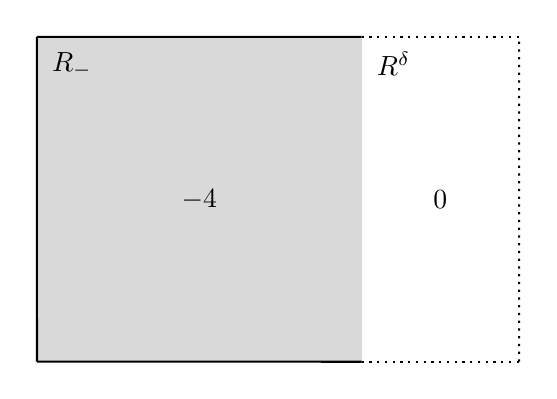
\begin{tikzpicture}[scale=0.8]
\node (A) at (-4,-2) {};
\node[right=4 of A.center] (B) {};
\node[right=6 of A.center] (O) {};

\node[above=4 of A.center] (A') {};
\node[above=4 of B.center] (B') {};
\node[above=4 of O.center] (O') {};

\fill[top color=gray!30, bottom color=gray!30] (A.center) rectangle node{$-4$} (B'.center);

\draw[thick] (A.center) -- (A'.center);
\draw[thick] (A.center) -- (B.center);
\draw[thick] (A'.center) -- (B'.center);

\node at ($(B)!0.5!(O')$) {0};

\node[below right=0.1 of A'.center] {$R_{-}$};
\node[below right=0.1 of B'.center] {$R^{\delta}$};

\draw[thick, dotted] (B.center) -- (O.center);
\draw[thick, dotted] (B'.center) -- (O'.center);
\draw[thick, dotted] (O.center) -- (O'.center);
\end{tikzpicture}
\end{minipage}
\hfill
\begin{minipage}{0.30\textwidth}
\small
\begin{align*}
R_{-} &= (-1,0)\times\left(-\tfrac12,\tfrac12\right), \\
R^{\delta} &= (0,\delta)\times\left(-\tfrac12,\tfrac12\right).
\end{align*}
\end{minipage}
\caption{Decomposition of the domain \( \Omega \) into subregions \( R_{-} \) and \( R^{\delta} \).
Solid lines indicate Dirichlet boundary conditions, while dotted lines correspond to Neumann (free) boundaries.}
\label{pic:pureinsulation_neumann}
\end{figure}
As a representative example, we consider the rectangular domain 
\[
\Omega = (-1,\delta)\times\left(-\tfrac12,\tfrac12\right), \qquad \delta \geq 0.
\] 
shown in Figure \ref{pic:pureinsulation_neumann}.
Homogeneous Dirichlet boundary conditions are imposed on
\[
\Gamma_D := \{ x \in \partial\Omega : x_1 \leq 0 \},
\]
and homogeneous Neumann boundary conditions on the remaining part
\[
\Gamma_N := \partial\Omega \setminus \Gamma_D.
\]
As \( \delta \to 0^+ \), the Neumann boundary degenerates to the vertical edge \( x_1 = 0 \).



The minimal eigenvalue and the associated eigenvector for \( \delta = 1 \) are shown in Figure~\ref{fig:min_eigenvector_neumann_full}. We observe a pronounced concentration of the determinant near the interface between \( R_{-} \) and \( R^{\delta} \).

To further investigate this effect, the domain is partitioned into layers in the \( x_1 \)-direction, and the contribution of the gradient term to the total energy is evaluated and normalized to one. Figure~\ref{fig:gradient_distribution} shows that the gradient part of the energy is likewise concentrated in a narrow region near the same interface.

\begin{figure}
    \centering
    \includegraphics[width=\textwidth]{minimal_eigenvector_neumann_full2.png}
    \caption{Components of \( \varphi_{\min} \) (first two columns) and \( \det(\nabla \varphi_{\min}) \) (third column) for \( c = -4 \) and \( \delta = 1\) on the mesh with 8192 triangles.}
    \label{fig:min_eigenvector_neumann_full}
%\end{figure}
%\vspace{0.5cm}
%\begin{figure}[H]
    \centering
    \includegraphics[width=0.69\textwidth]{distribution_of_gradients_level4.pdf}
    \caption{Distribution of the gradient contribution $|\nabla \varphi_{\min}|^2$ across \( x_1 \)-layers for \( c = -4 \) and \( \delta = 1 \) at level~4 mesh with 8192 triangles. Altogether, there are 64 \( x_1 \)-layers.}
    \label{fig:gradient_distribution}
%\end{figure}
%\begin{figure}
%\vspace{0.5cm}
    \centering
    \includegraphics[width=0.8\textwidth]{minimal_eigenvector_neumann.png}
  %  \vspace{0.3cm}
%    \includegraphics[width=\textwidth]{minimal_eigenvector_neumann_minus3.png}  
    \caption{Components of \( \varphi_{\min} \) for \( c = -4 \) and \( \delta = 0\) on the level 4 mesh with 4032 triangles.
  %  Components of the eigenvector \( \varphi_{\min} \) at level~4 mesh refinement for \( \delta = 0 \) with \( c = -4 \)
    %(top) and \( c = -3 \) (bottom).
    }
    \label{fig:min_eigenvector_neumann}
\end{figure}
In the limiting case \( \delta = 0 \), the minimal eigenvector localizes near the interface \( x_1 = 0 \), exhibiting boundary-dominated behavior as a consequence of the degeneration of the Neumann boundary; see Figure~\ref{fig:min_eigenvector_neumann}.

\vspace{0.5cm}
\noindent
{\bf Data availability statement}\\[1mm]
\noindent The MATLAB code used to generate the numerical results is available for download at
%\vspace{-3mm}
\begin{center}
\url{https://www.mathworks.com/matlabcentral/fileexchange/130564} .
\end{center}
\bigskip 
\noindent
{\bf Acknowledgment}\\[1mm]
    \noindent MK and JV were partially supported by the GA\v{C}R project 23-04766S; MK was also supported by the subsequent GA\v{C}R project 26-21585K. The authors thank JB and the Department of Mathematics at the University of Surrey for their hospitality. JB gratefully acknowledges the hospitality of MK, JV, and the \'{U}TIA, Czech Academy of Sciences, during his visits.

\begin{comment}
\subsubsection{Nonhomogeneous Dirichlet boundary condition on the part of the boundary}

\begin{figure}[h]
    \centering
    \includegraphics[width=0.99\textwidth]{solutionLinearSystem_nonhomog.png}
    
     \includegraphics[width=0.99\textwidth]{solutionLinearSystem_nonhomog_more3.png}
   \caption{Components of the minimizer (top). Bottom row: the $f$ distribution (left), energy densities (middle), and the deformed mesh (right).}
    \label{fig:minimizer}

 \includegraphics[width=0.99\textwidth]{solutionLinearSystem_nonhomog_more2.png}
    
\end{figure}    
\end{comment}



\begin{comment}

The command for the title is: \verb#\title#.
The \verb#\maketitle# command must be put after the abstract.


\subsection{Citations}

The bibliography must be built using bibtex. A sample of a bibtex file
\texttt{samplebib.bib} is with this sample.

The references must be refered to in the article by using the
\verb#\cite# command, which produces for example \cite{KNU} or
\cite{LL} (see also the comments in \texttt{samplebib.bib}).


\section{Figures}

The article being compiled with pdflatex, the figures should also be
in PDF (esp. for vector graphics, bitmap graphics should be of good
enough quality and can be PNG or JPEG). The inclusion of the figure is
done using the following commands.

The parameter \emph{xxx}, a real number between $0.0$ and $1.0$, indicates the
width the figure should take in the page.
One can refer to the figure with \verb+\ref{refname}+, which gives
for example: 

 Figure \ref{fig:exmp} is an example of figure.

 \begin{figure}[tbp]
 \includegraphics[width=0.4\linewidth]{Logo_Academie_grisfonce.pdf}
 \caption{Example of figure.}
 \label{fig:exmp}
 \end{figure}


 To refer to a specific definition, theorem, etc.,
 put \verb+\label{labelname}+ inside the corresponding environment and use
 \verb+\ref{labelname}+ in text to point to this definition, theorem,
 etc.

Here is an example:
\begin{theorem}\label{th:true}
  Most theorems are true.
\end{theorem}

\begin{proof}
  Th. \ref{th:true} is obviously true.
\end{proof}

\begin{exam}\label{ex:good}
  This should look like a good example.
\end{exam}

\begin{rema}
  Can an example like Ex.~\ref{ex:good} give some insight in
  Th.~\ref{th:true}'s proof?
\end{rema}




% The next command determines the bibliography style. Please do not
% change this.
\end{comment}
%\bibliographystyle{crplain}
\begin{thebibliography}{99}

%\bibitem{acerbi-fusco} E. Acerbi and N. Fusco. Semicontinuity problems in the calculus of variations. {\it Arch. Ration. Mech. Anal.} {\bf 86} (1984),  125-–145. 
%\bibitem{alibert-dacorogna} J.-J. Alibert, B. Dacorogna. An example of a quasiconvex function that is not polyconvex in two dimensions. {\it Arch. Ration. Mech. Anal.} {\bf 117}  (1992), 155--166.
%\bibitem{AIM} K. Astala, T. Iwaniec, G. Martin.   Elliptic Partial Differential Equations and Quasiconformal Mappings in the Plane.  Princeton Mathematical Series (Vol. 48).  Princeton University Press, 2009.

\bibitem{Ba77} J. M. Ball: Convexity conditions and existence theorems in nonlinear elasticity.  {\it Arch. Rat. Mech. Anal.},  {\bf 63}, no. 4 (1977), 337--403.
%\bibitem{bama}
J. M. Ball, J. Marsden. Quasiconvexity at the boundary, positivity of the second variation and elastic stability. {\it Arch.~Rat.~Mech.~Anal.} {\bf 86} (1984), 251--277. 

%\bibitem{Ball-Zhang}
%J. M. Ball, K. Zhang. Lower semicontinuity of multiple integrals and the Biting lemma. {\it Proc. Roy. Soc. Edinburgh} {\bf 114A} (1990), 367--379.

\bibitem{Bevan-14}
J. Bevan.  On double-covering stationary points of a constrained Dirichlet energy. {\it Ann. Inst. H. Poincar$\acute{\textrm{e}}$ Anal. Non Lin$\acute{\textrm{e}}$aire} {\bf 31} (2014),  391--411.

%\bibitem{BK19} J. Bevan, S. K\"{a}bisch.  Twists and shear maps in nonlinear elasticity:  explicit solutions and vanishing Jacobians.  Proc Roy. Soc. Ed. Sect. A 150 (2019) no. 1, 41-71. 

\bibitem{BKV23} 
J. Bevan, M. Kru\v{z}\'{i}k and J. Valdman. Hadamard's inequality in the mean.  Nonlinear Analysis {\bf(243)}, 
2024. https://doi.org/10.1016/j.na.2024.113523

\bibitem{BKV25} 
J. Bevan, M. Kru\v{z}\'{i}k and J. Valdman. New applications of Hadamard-in-the-mean inequalities to incompressible variational problems, Calculus of Variations and Partial Differential Equations {\bf(64)}, 259 (2025).

\bibitem{dacorogna} B. Dacorogna. {\it Direct Methods in the Calculus of Variations.} 2nd ed. Springer Science+Business Media, 2008. 

%\bibitem{dacorogna-marcellini}
B. Dacorogna, P. Marcellini. {\it Implicit Partial Differential Equations.}  Progress in nonlinear
differential equations and their applications 37, Birkh\"{a}user, Boston, 1999.

%\bibitem{FZ05} D. Faraco, K. Zhong.  Geometric rigidity of conformal matrices.   Ann. Scuola. Norm. Sup. Pisa Cl. Sci. (5) Vol. IV (2005), 557--585. 

\bibitem{BD22} M. Dengler, J. Bevan. A uniqueness criterion and a counterexample to regularity in an incompressible variational problem. Arxiv:2205.07694, 2022. 

%\bibitem{NPV2012} E. Di Nezza, G. Palatucci, E. Valdinoci.  Hitchhiker's guide to the fractional Sobolev spaces.  { \it Bulletin des Sciences Math\'{e}matiques.} {\bf 136} (2012), 521--573.

%\bibitem{evans1998}
%L.C. Evans. Partial Differential Equations. AMS Providence,  1998.
%\bibitem{F03} D. Faraco.  Rigidity of sets of matrices, In: "Future Trends in Geometric Functions Theory", Rep. Univ. Jyv\"{a}skyl\"{a} dep. Math. Stat., Vol. 92,  Univ. Jyv\"{a}skyl\"{a}, Jyv\"{a}skyl\"{a}, 2003. 



%\bibitem{fmp}
I. Fonseca, S. M\"{u}ller, P. Pedregal. Analysis of concentration and oscillation effects generated by gradients. {\it SIAM J. Math. Anal.} {\bf 29} (1998), 736--756.

\referee

\bibitem{GiaquintaGiusti1982} M. Giaquinta and E. Giusti.  On the regularity of minima of variational integrals. {\it Acta Math.} {\bf 148} (1982), 31--46.

%\bibitem{iwaniec}
T. Iwaniec. Nonlinear Cauchy-Riemann operators in $\R^n$
{\it Trans. AMS} {\bf 354} (2002),   1961-–1995.

\bibitem{iwaniec-lutoborski-ARMA}
 T. Iwaniec, A. Lutoborski. Integral estimates for null Lagrangians. {\it Arch. Ration. Mech. Anal.} {\bf  125} (1993), 25--79.

 \bibitem{iwaniec-lutoborski-SIMA}
 T. Iwaniec, A. Lutoborski. Polyconvex functionals for nearly conformal deformations. {\it SIAM J. Math. Anal.}
 {\bf 27} (1996), 609--619.

 
 \bibitem{john}
 F. John. Uniqueness of non-linear elastic equilibrium for prescribed boundary displacements and sufficiently small strains. {\it Comm. Pure Appl. Math.} {\bf XXV} (1972), 617--634. 


%\bibitem{kalamajska-kruzik} A. Kalamajska, M. Kru\v{z}\'{\i}k. Oscillations and concentrations in  sequences of gradients. {\it ESAIM Control Optim. Calc. Var.} {\bf 14} (2008), 71--104.

%\bibitem{kroemer}
%S. Kr\"{o}mer. On the role of lower bounds in characterizations
%of weak lower semicontinuity of multiple integrals. {\it Adv. Calc. Var.}  {\bf 3} (2010), 387–-408.

\bibitem{mielke-sprenger}
A. Mielke, P. Sprenger. Quasiconvexity at the boundary and a simple variational formulation of Agmon's condition. {\it J. Elast.} {\bf 51} (1998),  23--41.

%\bibitem{mova}
%A. Moskovka, J. Valdman. Fast MATLAB evaluation of nonlinear energies using FEM in 2D and 3D: nodal elements. {\it Applied Mathematics and Computation} {\bf 424},  (2022) 127048.

%\bibitem{morrey}
%C.B. Morrey: {\it Multiple Integrals in the Calculus of Variations.}  Springer, Berlin, 1966.
\bibitem{Mo66}  C. B. Morrey, Jr.  Multiple integrals in the calculus of variations. Reprint of the 1966 edition. Classics in Mathematics. Springer-Verlag, Berlin, 2008. 

\bibitem{neff}
D.Y. Gao, P. Neff, I. Roventa, C. Thiel. On the convexity of nonlinear elastic energies in  the right Cauchy-Green tensor. {\it J. Elasticity} {\bf 127} (2017), 303--308.

%\bibitem{Palka} B.W. Palka. {\it An Introduction to Complex Function Theory.} Springer, UTM. 1991.
%\bibitem{Pedregal}
%P. Pedregal. {\it Parametrized Measures and Variational Principles.}  Birkh\"{a}user, Basel, 1997. 

\bibitem{spector}
J. Sivaloganathan, S.J. Spector. On the uniqueness of energy einimizers in finite elasticity. {\it J. Elast.} {\bf 133} (2018), 73--103. 

\bibitem{spector2}
D.E. Spector, S.J. Spector. Uniqueness of equilibrium with sufficiently small strains in finite elasticity. {\it Arch. Ration. Mech. Anal.} {\bf 233} (2019), 409--449.\ 
\end{thebibliography}
%This calls all references from the .bib
\nocite{*}

%  This inserts the bib file
%\bibliography{samplebib}


\end{document}










